\documentclass[border={-2mm -2mm -2mm -2mm}]{standalone}
\usepackage{tikz}
\usepackage{inconsolata}
\usepackage{xcolor}
\usetikzlibrary{calc,positioning,backgrounds}

%\definecolor{bg}{rgb}{1,1,0.9}
%\definecolor{node}{rgb}{0.4,0.4,0.3}
%\definecolor{edgel}{rgb}{0.7,0.7,0.8}
%\definecolor{edged}{rgb}{0.3,0.3,0.4}

%\definecolor{bg}{rgb}{0,0.2,0.2}
%\definecolor{node}{rgb}{0.5,0.5,1}
%\definecolor{edgel}{rgb}{0.3,0.3,0.2}
%\definecolor{edged}{rgb}{0.9,0.9,0.4}

\definecolor{bg}{HTML}{2E4052}
\definecolor{node}{HTML}{E3D8F1}
%\definecolor{edgel}{HTML}{439A86}
%\definecolor{edged}{HTML}{FFC857}
\definecolor{edgel}{HTML}{439A86}
\definecolor{edged}{HTML}{439A86}

\tikzset{
  arrout/.style = {<-,> = latex,pos=0.64}, 
  lab/.style = {fill=bg,font=\ttfamily\bfseries,inner sep=0.5pt},
  arrin/.style = {->,> = latex,pos=0.36},
  entity/.style = {draw,thick,fill=node,node,font=\ttfamily\bfseries,text=edged,circle,inner sep=0.4mm},
  arr/.style = {draw = none,edgel,thin},
  arrd/.style = {edged,very thick}
}
\newlength{\hgap}
\setlength{\hgap}{0.13cm}

\begin{document}
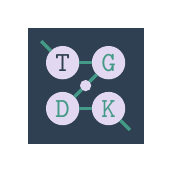
\begin{tikzpicture}[background rectangle/.style={fill=bg}, show background rectangle]
\node[entity] (c) {};

\node[entity,anchor=mid,above left=\hgap of c] (t) {\textcolor{bg}{T}}
  edge[arr] (c);
  
\node[entity,anchor=mid,above right=\hgap of c] (g) {G}
  edge[arrd] (c)
  edge[arrd] (t);
  
\node[entity,anchor=mid,below left=\hgap of c] (d) {D}
  edge[arrd] (c)
  edge[arr] (t);

\node[entity,anchor=mid,below right=\hgap of c] (k) {K}
  edge[arr] (c)
  edge[arr] (g)
  edge[arrd] (d);

\coordinate[below right=1.33\hgap of k] (kc) {}
  edge[arrd] (k);

\coordinate[below left=1.33\hgap of d] (dc) {}
  edge[arr] (d);

\coordinate[above left=1.33\hgap of t] (tc) {}
  edge[arrd] (t);

\coordinate[above right=1.33\hgap of g] (gc) {}
  edge[arr] (g);

%\coordinate (dk) at ($(kc)!0.5!(dc)$) {}
%  edge[arr] (d)
%  edge[arrd] (k);
%
%\coordinate (td) at ($(tc)!0.5!(dc)$) {}
% edge[arr] (d)
% edge[arrd] (t);
%
%\coordinate (tg) at ($(tc)!0.5!(gc)$) {}
% edge[arr] (g)
% edge[arrd] (t);
%
%\coordinate (gk) at ($(gc)!0.5!(kc)$) {}
% edge[arr] (g)
% edge[arrd] (k);

%\node[entity,fill=blue!50!black,right=\hgap of i] (c) {C}
%  edge[arrout] node[lab] {J} (i);
%  
%\node[entity,fill=red,right=\hgap of c] (g) {G}
%  edge[arrout] node[lab] {K} (c)
%  edge[arrin,font=\ttfamily,bend left=55,pos=0.5] node[lab,font=\ttfamily] {21} (i)
%  edge[arrout,bend right=55,pos=0.5] node[lab,font=\ttfamily] {20} (i);
\end{tikzpicture}
\end{document} 